
\section{Introduction}
In this  Section the  proposed  methodology of this  project will be discussed this will cover the  following:
\begin{enumerate}
    \item The Procedure of the project
    \item The Additional reserach
    \item The setup of the raspberry pi
    \item The Model Development
    \item The Data Analysis Methods
    \item The validity and reliability 
    \item The Limitations and Delimitation
    \item The timeline
\end{enumerate} 
\section{Setup of raspberry pi}
Firstly once you have  your pi  heres  a  quick  guide to setup the pi are  the following:
\begin{enumerate}
    \item once you unpack the  pi be sure  to  connect keyboard mouse  and hdmi cable
    \item next on a computer you must download the  raspberry pi imager and  selet the  64 bit  recommned os 
    \item once u have os set simpley put the  mircosd card  into  the pi once the  pi is  setup you can make sub dirrys for this project type the  following:
    \begin{verbatim}
        git clone https://github.com/mistaherd/meshnetwork_in_forest.git
    \end{verbatim}
    this  will downlaod the  nessary  eniroment for  setinng up the  pi  intiall this will have to built out  through the  process of  the   project look at the timeline Section
    \item next simply follow the ReadME.md file  to  understand  how  to setup the py
\end{enumerate}


\section{Additional  Research}
In this section will discuss any extra research done on the project.
in this section we will discuss the following:
\begin{enumerate}
    \item ADC
    \item Radio module
\end{enumerate}
\subsection{ADC}
The MCP3008 was not  available when ordering parts,Another  part for this was choosen which is the  DFR0553 which has the following:
\begin{enumerate}
    \item a supply voltages(VCC) of 3.3 to 5 v
    \item Analog signal  detection 0 to 5v
    \item 4 analog chanel's
    \item resolution of 16 bits
    \item Operating current of 3mA
\end{enumerate}
\subsection{Radio module}
for  this  section we want  to keep  the following in mind :
\begin{enumerate}
    \item We want a module that will send  and  received data
    \item we don't  want  an  expensive solution due  to wanting to  have  multiple nodes
    \item must we pick a standard? 
    \item what module has  an open source project on it 
    \item how do we  set up  a   mesh network with this 
\end{enumerate}
\subsubsection{Do we need a radio standard?}
Lets assume we communicate with two pi via wires  we know that an interference will occur when  we  commutation that is wireless
we can have multiple cases where interference can  occur these are  the following:
\begin{enumerate}
    \item the signal being reflected of objects such as  trees
    \item the signal can reach the  receiver due to an object blocking the antenna
    \item the signal isn't  power to be picked up by the receiver
\end{enumerate}
one essential part of this project is the  ability to have  our nodes have an address to set this up
from a communication preceptive we could develop this when there is open source project that has sorted out the routeing for  you.
only issue with this approach is if there is any issues that come from the open source project we will inherit the bugs
with this in mind the following standards were found
\begin{enumerate}
    \item LoRa
\end{enumerate}
\subsubsection{LoRa}

In \cite{Wu_Liebeherr_2023} lora is used that will organize sensor
data from all nodes in the spanning tree toward the root(laptop /PC) this can be show by the  following:
\begin{figure}[h!]
    \centering
    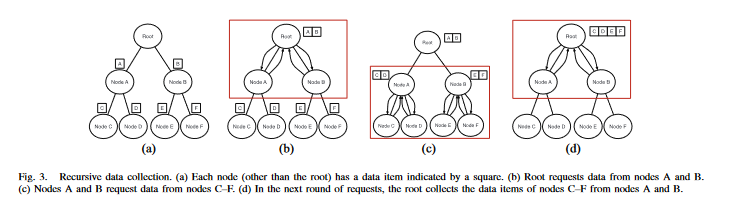
\includegraphics[width=0.5\linewidth]{Images/lora_example_routing_proto.png}
    \caption{protocol Wu used(wu\_lie et.al,2023:16705)}
    \label{protocol Wu used(wu_lie et.al,2023:16705)}
\end{figure}  
this proves it possible  to make a  mesh network using Lora.
\par 
from looking online Lora has more projects that are open source meaning we can use it.freely for example 
\par
Lora is uses spread spectrum modulation, In \cite{2003_Information_2023} spread spectrum is apparent in Shannon's theorem which states the channel capacity C the upper limit on the information rate of data that can be communciated at a lower error rate through the received signal power S:
$$C=B\log_2(1+\frac{S}{N})$$
Where B is the is the bandwidth of the channel in hertz.Where the bandwidth is:
$$B=F_{max}-F_{min}$$
spread spectrum  creates a pseudo-random code sequence that modulates the data signal  which will determine the  how  the signal is  spread out.

To simulate the system we can use the following FIR response  as an example 
\begin{figure}[h!]
    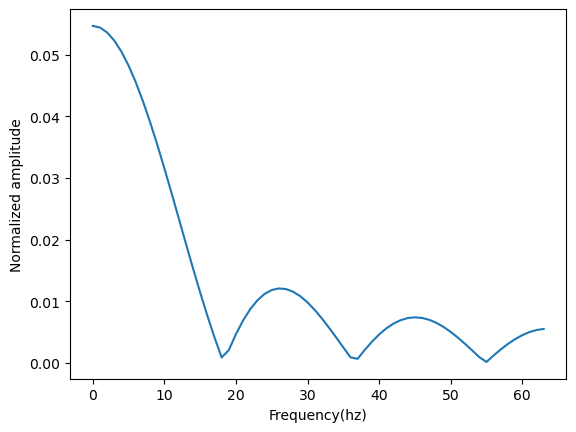
\includegraphics[width=0.5\linewidth]{Images/FIR_response.png}
    \caption{sample graph of a FIR response}
    \label{sample graph of a FIR response}

\end{figure}
in a given  medium  of  transmit each bandwidth is the length the of the  sinc-roll-off which degrade depends on the  impulse response in this given bandwidth channels are separated in the same fashion .
\subsection{What is  the difference  between a  port and a channel}
\newpage
\subsubsection{Why the MM2 Series 900 MHz wasnt picked}
When ordering the parts for  this module issues where due to company not selling the product to  enterprise-level businesses so then two alternative radio modules were found:
\begin{enumerate}
    \item SB Components LoRa HAT for Raspberry Pi
    \item RPIZ SHD LORA433 Raspberry Pi Shield - LoRa, 433 MHz, SX1268
\end{enumerate}
when we compare these we get the following table:

\begin{table}[h!]
    \scalebox{0.45}{
        \begin{tabular}{|l|l|l|l|l|l|l|l|l|}
            \hline
            \rowcolor[HTML]{343434} 
            \multicolumn{1}{|c|}{\cellcolor[HTML]{343434}\textbf{Modules}} & \multicolumn{1}{c|}{\cellcolor[HTML]{343434}\textbf{Tx/RX Voltage}} & \multicolumn{1}{c|}{\cellcolor[HTML]{343434}\textbf{Frequency}} & \multicolumn{1}{c|}{\cellcolor[HTML]{343434}\textbf{Range}} & \multicolumn{1}{c|}{\cellcolor[HTML]{343434}\textbf{TX/RX power}} & \multicolumn{1}{c|}{\cellcolor[HTML]{343434}\textbf{Through put}} & \multicolumn{1}{c|}{\cellcolor[HTML]{343434}\textbf{Error detection}} & \multicolumn{1}{c|}{\cellcolor[HTML]{343434}\textbf{Rx sensitivity}} & \multicolumn{1}{c|}{\cellcolor[HTML]{343434}\textbf{Hopping channel}} \\ \hline
            SX1268 433M LoRa HAT & 5v & \begin{tabular}[c]{@{}l@{}}410.125$\sim$493.125MHz \\ or \\ 850.125$\sim$930.125MHz\end{tabular} & \begin{tabular}[c]{@{}l@{}}5KM(Sunny day; open area;\\  Antenna: AUX 5dBi,\\  Height 2.5m; \\ Air Speed: 2.4kbps)\end{tabular} & 11ma /100ma & 0.3Kbps & None & -147dBm@0.3Kbps (On air) & None \\ \hline
            SB Components LoRa HAT for Raspberry Pi & 5v & 915/868/433 MHz & 5km & 22dBm & 0.3Kbps & None & N/A & None \\ \hline
            \end{tabular}        
        }
        \caption{Comparing New Radio modules}
        \label{Comparing New Radio modules}
\end{table}
SB Components LoRa HAT for Raspberry Pi   was picked which has the according to its datasheet to install it onto  the pi the designer has to  




\section{Software Module Development}
This section is here to discuss the method we took  for  developing software  for the  following:
\begin{enumerate}
    \item Sensors 
    \item ADC
    \item Camera
    \item Radio module
    \item Memory management
    \item  TDD
\end{enumerate}
\subsection{Sensors}
This Section will discuss the following:
\begin{enumerate}
    \item DHT22
    \item AS312
    \item DFR0026
\end{enumerate}
To see the light sensor look on page \pageref{ADC section} 
\subsubsection{DHT22}
For this section we used the following libraries:
\begin{lstlisting}[style=mystyle]
#!/home/mistaherd/Documents/Github/meshnetwork_in_forest/env/lib/python3.11
import adafruit_dht 
import board
import pandas as pd  
\end{lstlisting} 
This uses the library from \href{https://github.com/mrmcwethy/Adafruit_CircuitPython_DHT}{this link}
\begin{enumerate}
    \item we define the our class
    \begin{lstlisting}[style=mystyle]
    class DHT22:
    ##Set DATA pin to pin 4
        def __init__(self):
            """this will setup the  data pin  for  DHT2"""
            # self.dhtDevice =adafruit_dht.DHT22(board.D4)
            self.dhtDevice =adafruit_dht.DHT11(board.D4)
            self.humidity=self.dhtDevice.humidity
            self.temperature=self.dhtDevice.temperature
    \end{lstlisting}
    In this class we have  define our DhT device as 11 seen as the DHT22 was  broken
    so we set  our gpio pin 4 and setup the variables that read the  sensor data
    \item Next we read the data from the following function.
    \begin{lstlisting}[style=mystyle]
        def Read_DHT22_data(self)-> tuple[float,float,str]:
        """This  will setup a DHT instance and  return the data from the sensor"""
        try:
            return self.temperature,self.humidity
        except RuntimeError as e:
            print(f"Error reading sensor: {e}")
            return None, None
    \end{lstlisting}
    this will  return out the  temperature and humidity if the sensor is not connected
    this  will return nothing . next  use the following: 
    \begin{lstlisting}[style=mystyle]
        if __name__ =="__main__":
            DHT22()
    \end{lstlisting}
\end{enumerate}
\subsubsection{AS312}
For this we import the following libraries:
\begin{lstlisting}[style=mystyle]
    #!/home/mistaherd/Documents/Github/meshnetwork_in_forest/env/lib/python3.11
    import RPi.GPIO as GPIO
    import time
\end{lstlisting}
\begin{enumerate}
    \item next  we set up our variables  in the class
    \begin{lstlisting}[style=mystyle]
    class AS312:
	def __init__(self):
		"connect the AS312 to pin 17"
		self.pin_number=17
		self.GPIO=GPIO
		self.GPIO.setmode(GPIO.BCM)
		self.GPIO.setup(self.pin_number,GPIO.IN)
		self.current_state=0
    \end{lstlisting}
    This sets current state as 0
    \item next  we detect  movement
    \begin{lstlisting}[style=mystyle]
        def read_state(self)->bool:
            time.sleep(0.1)
            self.current_state =bool(self.GPIO.input(self.pin_number))
            return self.current_state
    \end{lstlisting}

\end{enumerate}

\subsubsection{DFR0026}
\label{ADC section}
From the repository DFRobot_ADS1115 we do the following:
\begin{enumerate}
    \item import the libraries
    \begin{lstlisting}[style=mystyle]
        #!/home/mistaherd/Documents/Github/meshnetwork_in_forest/env/lib/python3.11
        from DFRobot_ADS1115 import ADS1115
        import time
    \end{lstlisting}
    \item Next we define our variables
    \begin{lstlisting}[style=mystyle]
    class DFR0026():
        def __init__(self):
            self.ADS1115_REG_CONFIG_PGA_6_144V        = 0x00 # 6.144V range = Gain 2/3
            self.ADS1115_REG_CONFIG_PGA_4_096V        = 0x02 # 4.096V range = Gain 1
            self.ADS1115_REG_CONFIG_PGA_2_048V        = 0x04 # 2.048V range = Gain 2 (default)
            self.ADS1115_REG_CONFIG_PGA_1_024V        = 0x06 # 1.024V range = Gain 4
            self.ADS1115_REG_CONFIG_PGA_0_512V        = 0x08 # 0.512V range = Gain 8
            self.ADS1115_REG_CONFIG_PGA_0_256V        = 0x0A # 0.256V range = Gain 16
            self.ads1115 = ADS1115()
            self.ads1115.set_addr_ADS1115(0x48)
            self.ads1115.set_gain(self.ADS1115_REG_CONFIG_PGA_6_144V)
            self.adc_channel=0
    \end{lstlisting}
    This configures all the pins  and set the associative gain
    \item Next read the analogue channel
    \begin{lstlisting}[style=mystyle]
        def read_voltage(self):
            return self.ads1115.read_voltage(self.adc_channel)
    \end{lstlisting}
\end{enumerate}
\newpage
\subsection{Camera}
Here are the steps for module development of the Camera:
\begin{enumerate}
    \item install the following libraries:
    \begin{lstlisting}[style=mystyle]
        #!/home/mistaherd/Documents/Github/meshnetwork_in_forest/env/lib/python3.11
        from picamera2 import Picamera2 ,Preview
        from time import sleep
        from datetime import datetime
    \end{lstlisting}
    \item we dine our class variables
    \begin{lstlisting}[style=mystyle]
    class Raspberry_Pi_VR_220:
        def __init__(self):
            """setup an instan  for the  camera"""
            self.timestamp=datetime.now().strftime("%Y-%m-%d_%H-%M-%S")
            self.fname ='/home/mistaherd/Documents/Github/meshnetwork_in_forest/Images_camera/{}.png'.format(self.timestamp)
            self.camera=Picamera2()
            self.camera_config=self.camera.create_preview_configuration()
            self.timeamount=2
    \end{lstlisting}
    \item  make the function for  takeing  a  picture
    \begin{lstlisting}[style=mystyle]
        def take_pic(self)-> str:
            """this will take  a picture from camera"""
            self.camera.configure(self.camera_config)
            self.camera.start_preview(Preview.QTGL)
            self.camera.start()
            sleep(self.timeamount)
            self.camera.capture_file(self.fname)
            return self.fname
    \end{lstlisting}
\end{enumerate}
\newpage
\subsection{Memory Management}
For this we want to  read data  and append and check it the memory size.Here are the following steps:
\begin{enumerate}
    \item  import the following  libraries:
    \begin{lstlisting}[style=mystyle]
        #!/home/mistaherd/Documents/Github/meshnetwork_in_forest/env/lib/python3.11
        import pandas as pd
        from DHT22 import DHT22
        from AS312 import AS312
        from DFR0026 import DFR0026
        import glob
        import re 
        import subprocess
    \end{lstlisting}
    \item define our class  senors
    \begin{lstlisting}[style=mystyle]
    class sensor_data:
        def __init__(self):
            self.dht22 = DHT22()
            self.humidity,self.temperature=self.dht22.Read_DHT22_data()
            self.AS312=AS312(17)
            self.motion_detected =AS312.read_state()
            self.DF0026 =DFR0026()
            self.light_value=self.DF0026.Read_data()
            self.fname="sensor_data.csv"
    \end{lstlisting}
    \item We write and append our data to  the csv file
    \begin{lstlisting}[style=mystyle]
        def write_append_csv(self):
		data = { "Timestamp" : self.timestamp,
			"Temperature(oc)" : self.Temperature,
			"Humidity(%)" : self.humidity,
			"Light(lux)" :self.light_value,
			"Motion Detected": self.motion_detected
			}
		df = pd.DataFrame(data)
		if glob.glob(self.fname):	
			df.to_csv(self.fname,mode='a' ,index=False,header=False)
		else:
			df.to_csv(self.fname,mode='w' ,index=False)
    \end{lstlisting}
    \newpage
    \item Next we define our variables for testing  memory
    \begin{lstlisting}[style=mystyle]
    class Memory_tester():
        def __init__(self):
            self.units={"K":10e3,"M": 10e6,"G":10e9}
            self.regex ="\d{4}\.\[0-9]{1,3}[K,M,G]"
            self.fname="../bash_scrpits/memorytest.sh" 
            self.output_bash=subprocess.check_output(["bash",self.fname],universal_newlines=True)
    \end{lstlisting}
    \item next we check our memory
    \begin{lstlisting}[style=mystyle]
        def check_memory(self):
            try:
                if re.search(self.regex,self.output_bash):
                    value,unit=match.group(0).split()
                    try:
                        return float(value)*self.units[unit]
                    except KeyError:
                        raise ValueError(f"unknown unit: {unit}")
                
            except subprocess.CalledProcessError as e:
                raise ValueError(f"Error running script:{e.output}")
    \end{lstlisting}
    \item  we then  make an error if its useing  20 percent memory
    \begin{lstlisting}[style=mystyle]
        def error_check(self):
            mem=self.check_memory()
            max=32*10e9
            if mem >= 0.2* max:
                raise MemoryError("memory on pi is about to  used up")
    \end{lstlisting}
    \item to make sure  our class run from another python file 
    \begin{lstlisting}[style=mystyle]
        if __name__=="__main__":
            sensor_data()
            Memory_tester()
    \end{lstlisting}
\end{enumerate}

\newpage
Fristly i want to made  some unit tests the aim of this  is the  following:
\begin{itemize}
    \item To make  test  that will be  there for  the  codeing  section of  the  project 
\end{itemize}
this section will discuss the  following for  testing:
\begin{enumerate}
    \item 1 x DHT22
    \item 1 x DFR0026
    \item 1 x AS312
    \item 1 x MM2 Series 900 MHz
    \item 1 x MCP3008
    \item 1 x Raspberry Pi VR 220 Camera
    \item  1 x Li-polymer Battery HAT 
    \item 1 x Turbo 1GB 
\end{enumerate}
\subsubsection{DHT22}
According to the  data sheet \cite{sparkfun} seen as  the data is   8 bits  and  the  range at which this   operates at  -40 to 80$^{o}$c for tempeature
meaning we have  at least  7 bit in the  exponent to  represent  the   measured value.
to represent  the  high  end of this  sensor i used the  following calculation:
$$ 2^6 +2^4 = 80$$ which mean  we have  a 2 bits dedicated to decimal place so the  high temperature to be 80.3$^{o}$c
for the  lowest temp we have 6 bits  to  represent  - 40 due to  2s complement  so lowest  will   be -40.3$^{o}C$
so with that  that  stablish we  must  make a  unit  that will do  the  following:
\begin{enumerate}
    \item Test if the  output is  a float
    \item Test the  high end of  the  temp sensor so it  reads  80.3 as  the highest
    \item Test for the  lowest   temp   around 
\end{enumerate}
be sure to follow  steps  for  folder  setup  follow instructions on page \pageref{folderstructure}.
we get the following sample code:
\begin{lstlisting}[style=mystyle,caption={sample test intial code}]
import unittest
from protest import Read_DHT22
class test_project_code(unittest.TestCase):
    def test_DHT_22_temp_output_type(self):
        self.assertIsInstance(Read_DHT22, float)
    def test_DHT22_temp_range(self):
        self.assertGreaterEqual(Read_DHT22,-30.3)
        self.assertLessEqual(Read_DHT22,80.3)
    
\end{lstlisting} 
This code import unitest . the from protest is  a python files  we can  install  functions from other python files this can be usefull for testing purposes
then we initalized a test class call Unittest.testcase our firstion fucntion of the class  we  check if the number of the output  is a float or not this is  for  testing  tempearture
the next function we test for  is the range i look at the datasheet online   this code is  simpley testing the  limits of the  DHT22
for  humidity  the Datasheet which ranges from 0 to 100 \%
we want to test for the following:
\begin{enumerate}
    \item Test if the  output is  a float
    \item Test if the  output ranges 0 to 100
\end{enumerate}
this lead to the  following code 
\begin{lstlisting}[style=mystyle,caption={sample test for DHT22}]
import unittest
from protest import Read_DHT22
class test_project_code(unittest.TestCase):
    hum,temp=Read_DHT22(2)
    def test_DHT22_output_type(self):
        self.assertIsInstance(Read_DHT22,tuple)
    #....

    def test_DHT22_hum_output_type(self):
        self.assertIsInstance(hum,float)

    def test_DHT22_hum_range(self):
        self.assertGreaterEqual(hum,0.0)
        self.assertLessEqual(hum,100.0)
\end{lstlisting}
seen as we expect our sensor to  print out a humdity and temp values we  set the  output to  a tuple 
to test for this we use isInstacne which will test if its a tuple
next we test for the  limits of the  humidity
\subsubsection{DFR0026 \& MCP3008}
According to the  datasheet \cite{ada} we must keep in mind  that this  componet is  connected to  an ADC 
this  will  give  me  the  following  test conditions:
\begin{enumerate}
    \item Test if  the output is a float

    \item Test  the  range of this  with the  upper limit being 5v 
    \item test the  lover limit being 0 
\end{enumerate}
\begin{lstlisting}[style=mystyle,caption={unit test for  DFR0026 and  MCP3008}]
    import unittest
    from protest import Read_DHT22,Read_MCP3008
    class test_project_code(unittest.TestCase):
    def test_DFR0026_MCP3008_out_type(self):
        self.assertIsInstance(Read_MCP3008,float)
    def test_DFR0026_MCP3008_out_range(self):
        self.assertLessEqual(5.0000000)
        self.assertGreaterEqual(0.0000000)
\end{lstlisting}
this code is in the same in theres of limits
\subsubsection{AS312}
for  this section  we  want our  tests  to  be  the following:
\begin{enumerate}
    \item test for type is boolean 
\end{enumerate}
we can  now add to the snipppet :
\begin{lstlisting}[style=mystyle,caption={unit test for AS312}]
    def test_AS312_out_type(self):
        self.assertIsInstance(Read_AS312,bool)
\end{lstlisting}
\textbf{Note : Don't forget to import read_as12 function from test file}
seen as  thhis is a motion sensor  our ouout will be true or false
\subsubsection{Raspberry Pi VR 220 Camera}
according to the  data sheet \cite{Camera}
we the  resoultion to  it uses is  1080p50 which is 1920x1080p so our  tests will have to  in copoarte  the  followoing:
\begin{enumerate}
    \item Test the  output shape  if open cv is  gonna  be  used 
    \begin{enumerate}
        \item test  the  amout of   elelecelm in the  3 dimesional   array 
    \end{enumerate}
    \item test the  file  type  is png
\end{enumerate}
this would lead me to the following code snippet.
\begin{lstlisting}[style=mystyle,caption={camera unit test}]
    def test_Raspberry_Pi_VR220_out_shape(self):
    self.assertEqual(Read_Raspberry_PiVR220.shape,(1920,1080,3))
\end{lstlisting}
this function check the  pixeal count or resoulkation
\subsubsection{Li-polymer Battery HAT}

\subsubsection{memory moduldes }
in this setion will dicuss the following:
\begin{enumerate}
    \item silicon power 32GB 
    \item Turbo 1GB
\end{enumerate}
for this  i will use  useing  a  bash script(see this on page \pageref{TDD sample bash}) and what we are doing is  testing  the size in a  certain range for the silicon  SD card
\begin{enumerate}
    \item  Turbo 1GB
    as from above we are  import the file at which where our functions live in code frist we import the function
    \begin{lstlisting}[style=mystyle,caption={si powerd SD snippnet }]
        import unittest
        from protest import Read_DHT22,Read_MCP3008,Read_AS312,Read_Raspberry_PiVR220,Read_Memory_module
    
        def Test_memory_module_turbo_1GB_size(self):
            #testing  turbo 1GB
            self.assertLessEqual(Read_Memory_module,1e9)
            self.assertGreaterEqual(Read_Memory_module,0)
    \end{lstlisting}
    then simply we call assert and greater than which sets the bounds of the   modes the 1e9 is a way to put $1 × 10^9$
    whcih output that will between 1GB and  0
    \item silicon power 32GB
\end{enumerate} 
\subsubsection{MM2 Series 900 MHz}

\subsubsection{conculsion}
The  intiall  draft  code  for  the  test  devlopemnt  si the  following
\begin{lstlisting}[style=mystyle,caption={Final draft test template}]
    # waiting for other sections 
\end{lstlisting}

\section{Data Analysis Methods}

Statistical and machine learning techniques are employed to analyze the data collected from both computational models and real-world sources. These techniques are used to identify patterns, trends, and relationships within the data.


\section{Validity and Reliability}

Validation of computational models is achieved through rigorous testing and evaluation. This involves comparing model predictions with real-world data and examining the sensitivity of the models to different parameters. Reliability is ensured through the use of standardized methods and procedures for data collection, analysis, and interpretation.

\section{Limitations and Delimitations}

The computational nature of the research introduces limitations due to the complexity of the systems being modeled and the potential for errors in modeling and data analysis. Moreover, the generalizability of the findings may be limited to the specific contexts and conditions considered in the research.

\section{Timeline}
The research  phase will be  conducted from 20/09/2023 to \today.The prosed impanation phase is from january till \today